\chapter{Realisierung}
\label{chap:Realisierung}
Dieses Kapitel beschreibt die Realisierung des Prototyps. Der Prototyp ist eine überarbeitete Version der Konzeptvariante 2, siehe Unterkapitel \ref{sec:var2}. Es mussten Änderungen bei verschiedenen Komponenten durchgeführt werden, diese werden im Unterkapitel \ref{sec:mechKomp} erläutert. In Abbildung \ref{fig:Gesamtbild} ist das realisierte Konzept ersichtlich.

\begin{figure}[H]
	\centering
	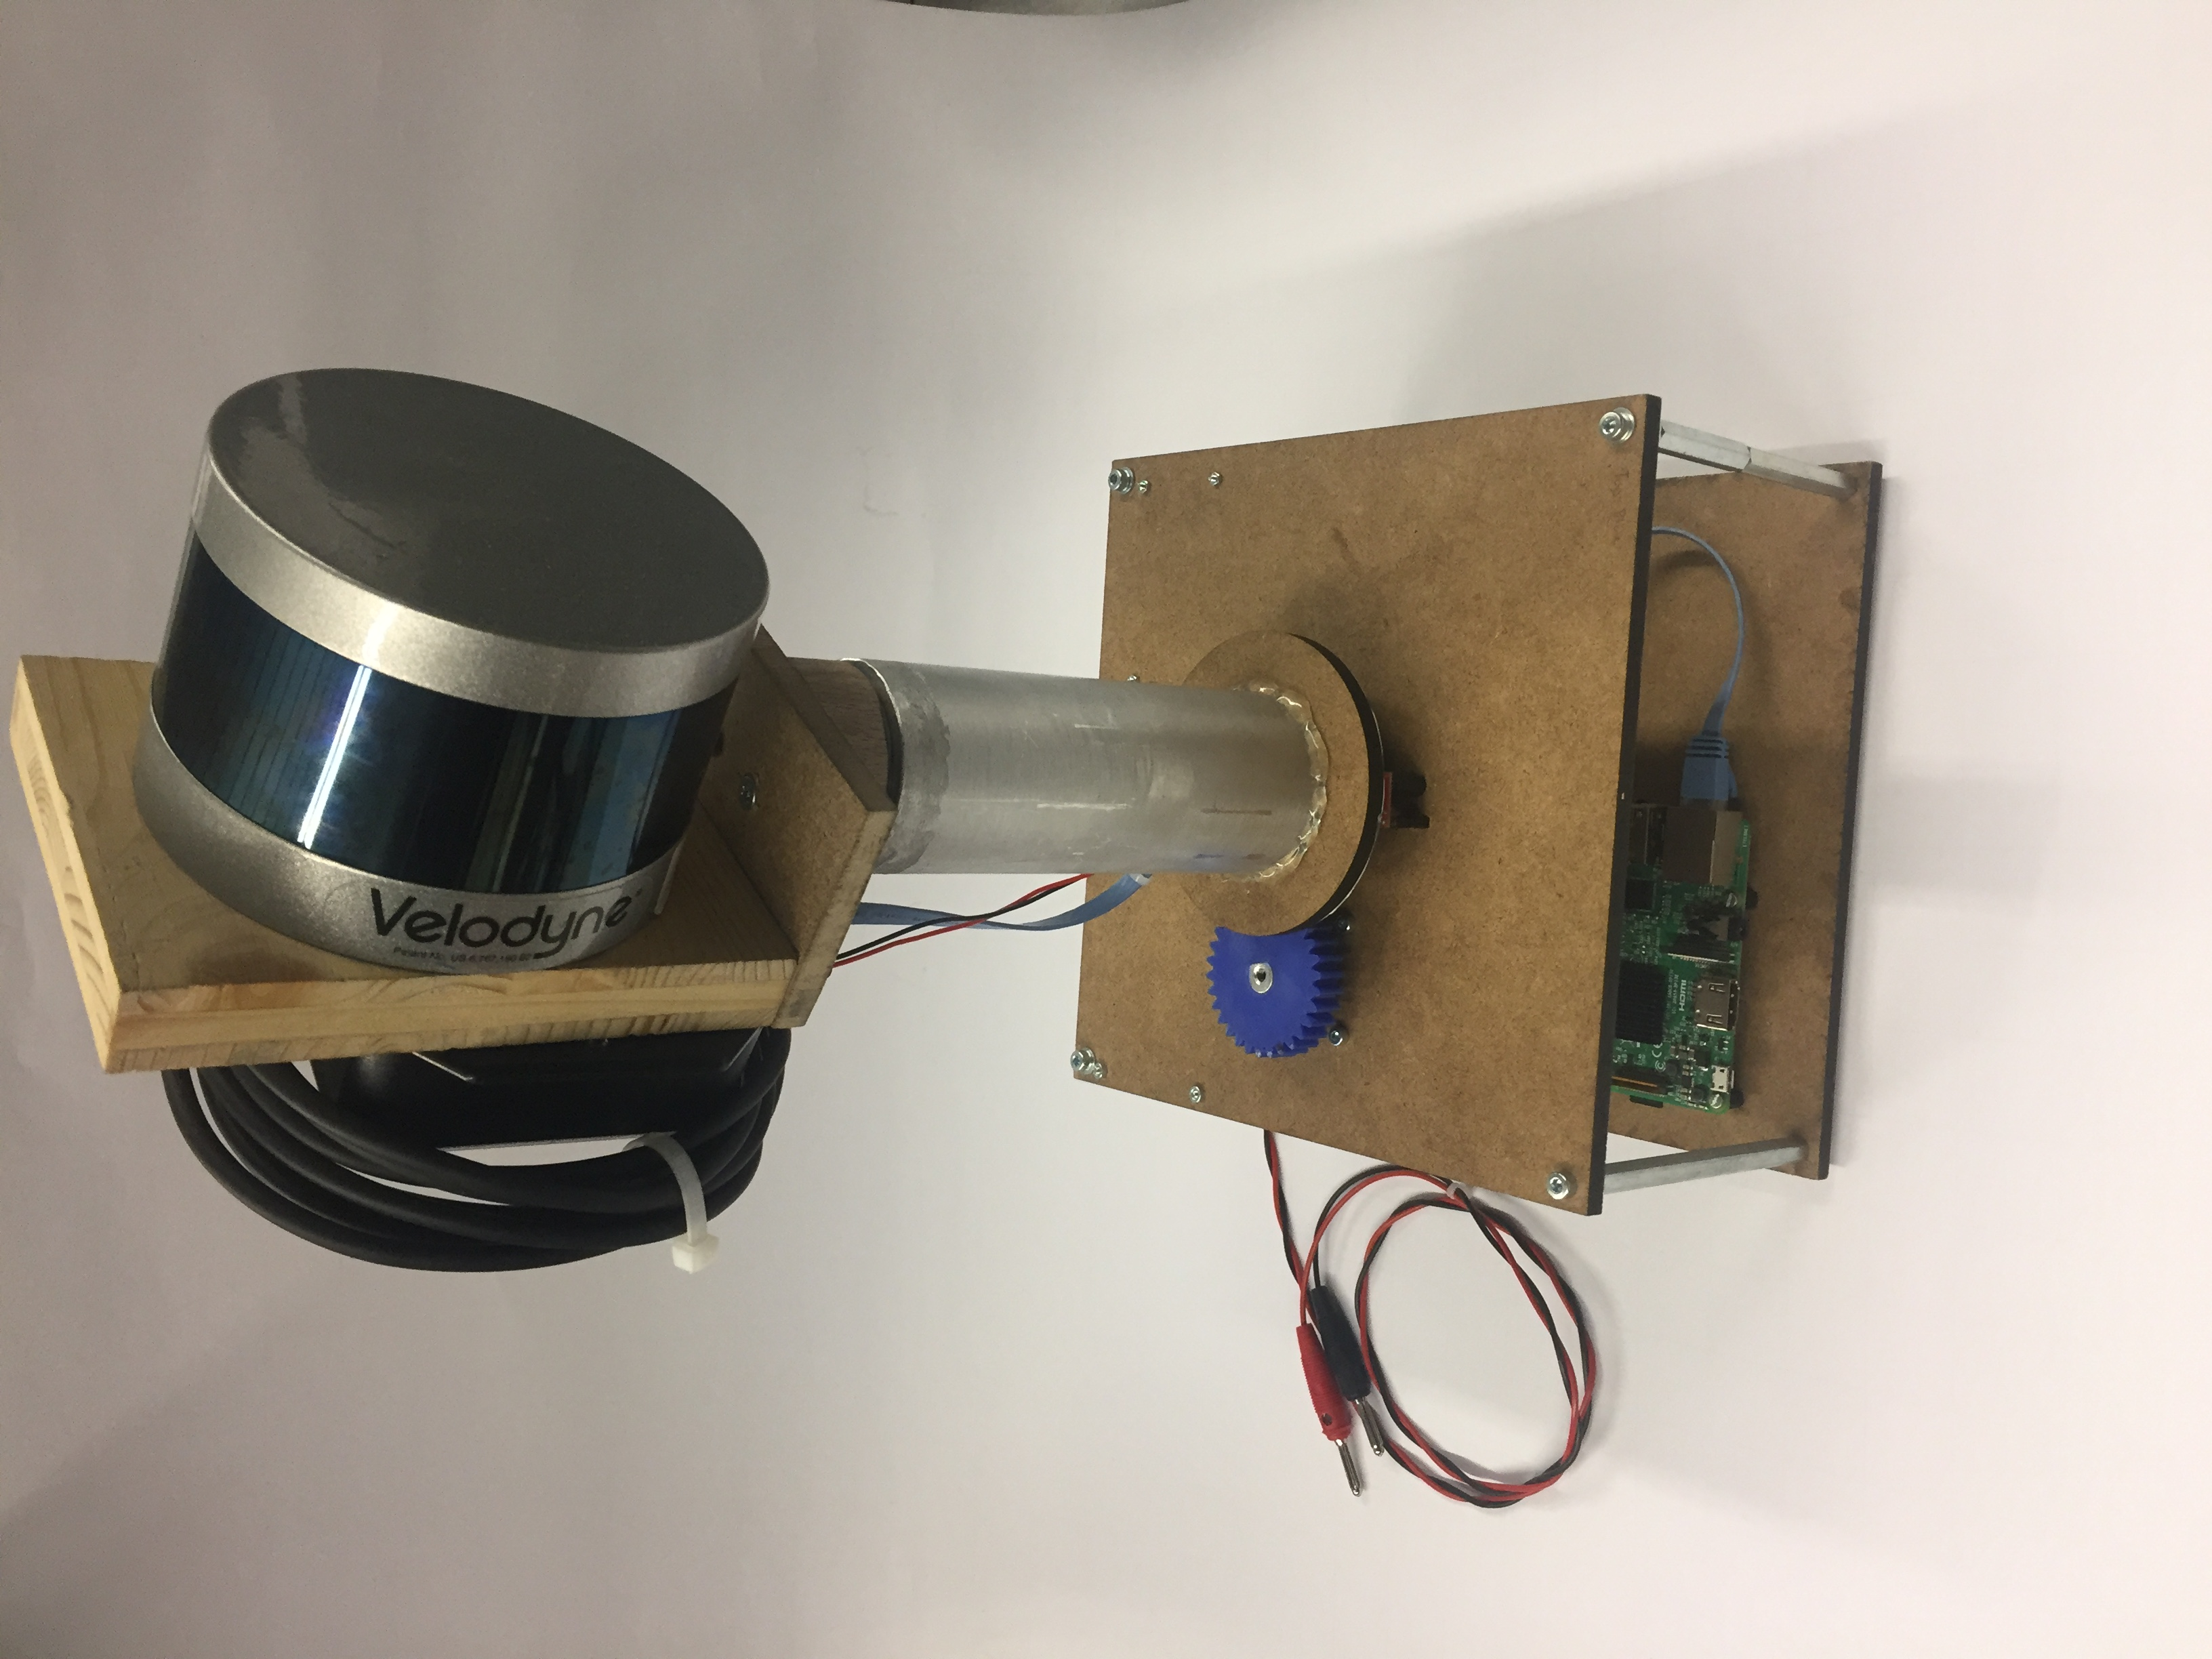
\includegraphics[angle=-90,width=0.58\textwidth]{resources/Gesamtbild.JPG}
	\caption[realisiertes Konzept]{realisiertes Konzept}
	\label{fig:Gesamtbild}
\end{figure} 


\section {Hardware}
\label{sec:Hardware}

Da beide Projekte, welche im Unterkapitel \ref{sec:Vorzeigeprojekte} eine endlos drehende Konstruktion nutzen, sowie die Aufgabenstellung im Anhang \ref{Pflichtenheft} eine drehende Konstruktion vorgibt, wurde eine endlos drehende mechanische Konstruktion angefertigt. 

\subsection {mechanische Komponenten \& Gehäuse}
\label{sec:mechKomp}

Um eine möglichst einfache und schnelle Lösung zu realisieren, wurden die mechanischen Komponenten nach Verfügbarkeit ausgewählt. Die Masse des Alurohrs und der Zahnräder waren größtenteils durch die verfügbare Grösse des Kugellagers gegeben. Das Kugellager wurde so gewählt, dass ein Ethernet RJ45 Stecker hindurchgeführt werden kann. Daraus ergibt sich einen Innendurchmesser von 22 mm und der entsprechende Aussendurchmesser von 44 mm.
Das Kugellager wurde direkt in das Alurohr gepresst und zusätzlich seitlich mit Schrauben verkeilt. Das Alurohr wurde mit einem Aussendurchmesser von 50 mm und einer Wandstärke von 3mm gewählt. Einerseits ist so der Innendurchmesser des Alurohrs passend zum Aussendurchmesser des Kugellagers und anderseits können bei dieser Wandstärke Gewinde geschnitten werden, damit Schrauben als Keil verschraubt werden können.

Der innere Ring des Kugellagers wurde auf den Kugellageradapter gesteckt. Dieser ist wiederum wie in Abbildung \ref{fig:mechKomp} an der Deckplatte befestigt. Somit lässt sich das Alurohr mit wenig Reibung drehen.

Die zwei Zanhräder wurden mit dem CAD-Tool OnShape gelayoutet und im FabLab mit einem 3D-Drucker erzeugt. Das grosse Zahnrad mit 48 Zähnen besitzt den Innendurchmesser 50 mm, welcher dem Alurohr entspricht. Dieses wurde auf das Alurohr gepresst. Das zweite Zahnrad ist im Verhältnis 1.5:1 kleiner und besitzt 32 Zähne. Die Übersetzung wurde so gewählt, dass die Komponenten mit genügend Abstand nebeneinander montiert werden können. Dieses Verhältnis muss bei der Softwareimplementierung berücksichtigt werden.

\begin{figure}[H]
	\centering
	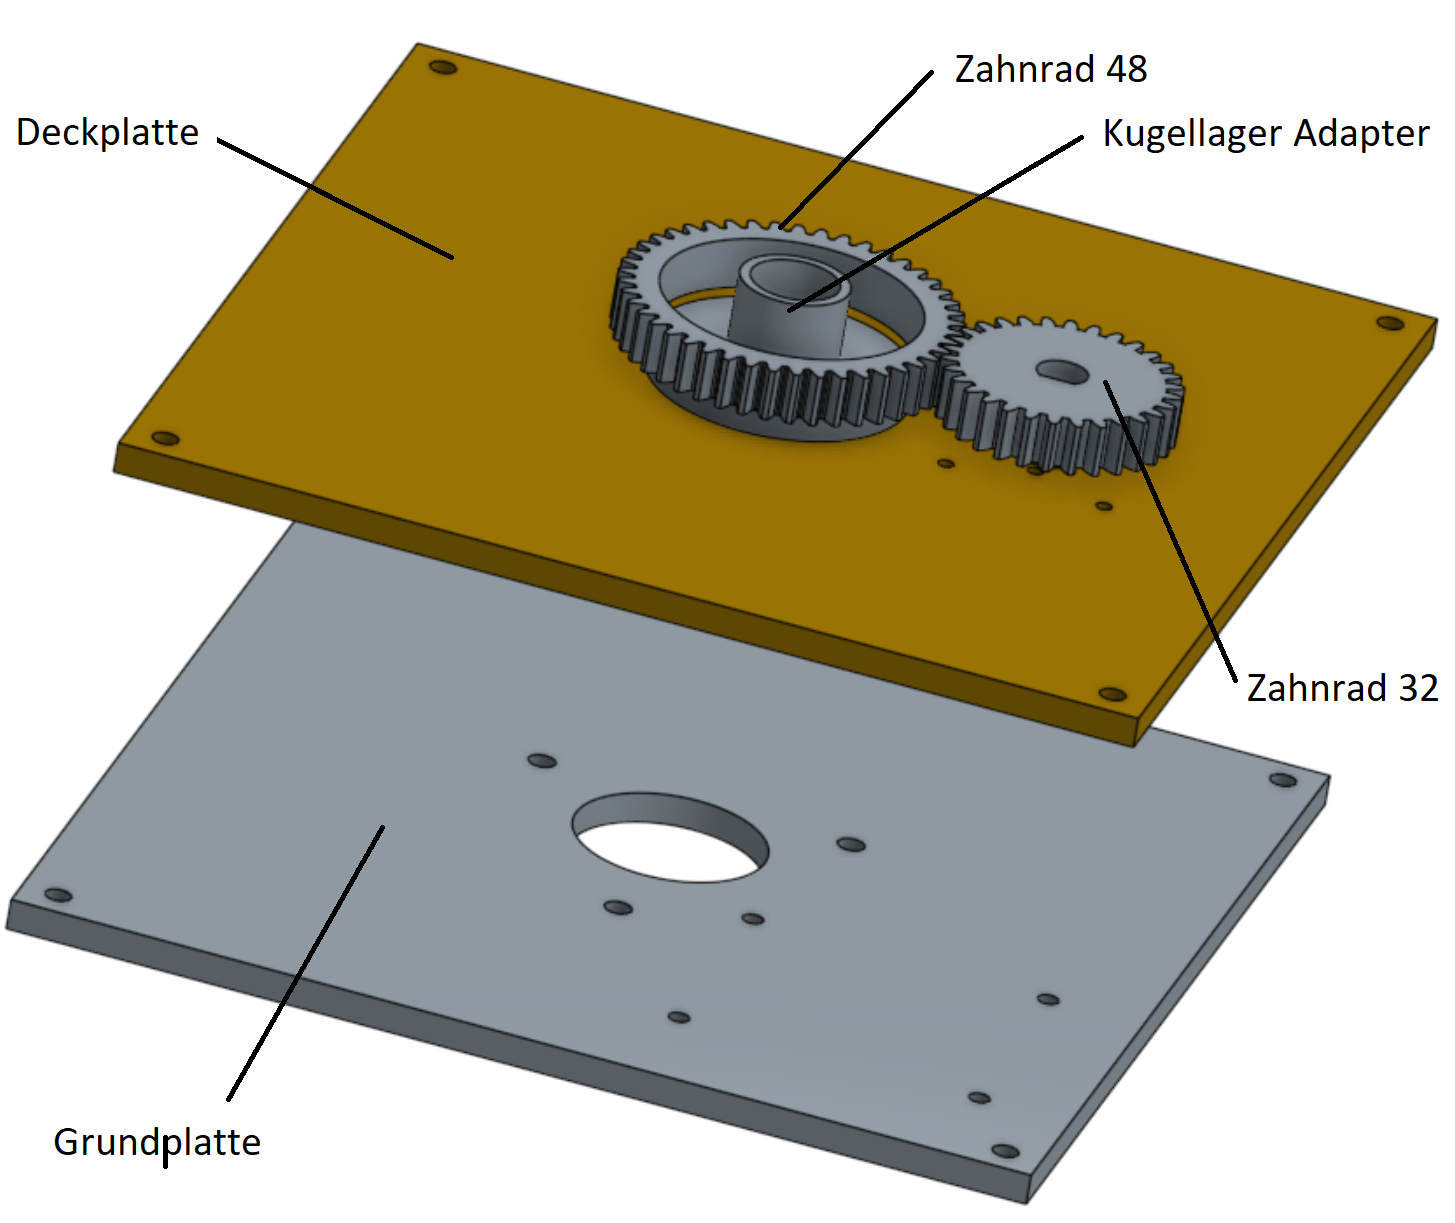
\includegraphics[width=0.8\textwidth]{resources/mechKomp2.PNG}
	\caption{gelayoutete Komponenten in OnShape}
	\label{fig:mechKomp}
\end{figure} 

Die Grösse der Platten wurde so gewählt, dass alle Komponenten dazwischen verbaut werden können. Daher wurden zwei MDF-Platten mit den Massen 200 mm x 200 mm x 6 mm (HxBxT) im FabLab erstellt. Die Grund- und Deckplatten wurden in OnShape gelayoutet und besitzen bereits vorgefertigte Löcher für die Montage der elektrischen Komponenten.

\subsection {elektrische Komponenten}
\label{sec:elekKomp}

Der Velodyne VLP-16 wurde auf einen rechtwinklige Konstruktion montiert, so dass der Lasermittelpunkt möglichst auf der Drehachse liegt. Die Interface Box wurde direkt gegenüber des Lasers montiert. Über den Schleifring führen eine 12 Volt Speisung und das Ethernetkabel direkt zu den erforderlichen Anschlüssen. Mit dieser Konfiguration lässt sich der Velodyne über die Zahnräder endlos drehen.

Die Nullposition wird mittels dem QRE 1113 und einem Hohlzylinder detektiert. Der Hohlzylinder ist dabei am rotierenden Alurohr befestigt. Der QRE 1113 ist mit dem Abstand von 2 mm unterhalb des Hohlzylinder fest montiert. Indem auf dem Hohlzylinder ein schwarzer Streifen auf eine weisse Oberfläche gedruckt ist, kann der Nullpunkt detektiert werden.

\begin{figure}[H]
	\centering
	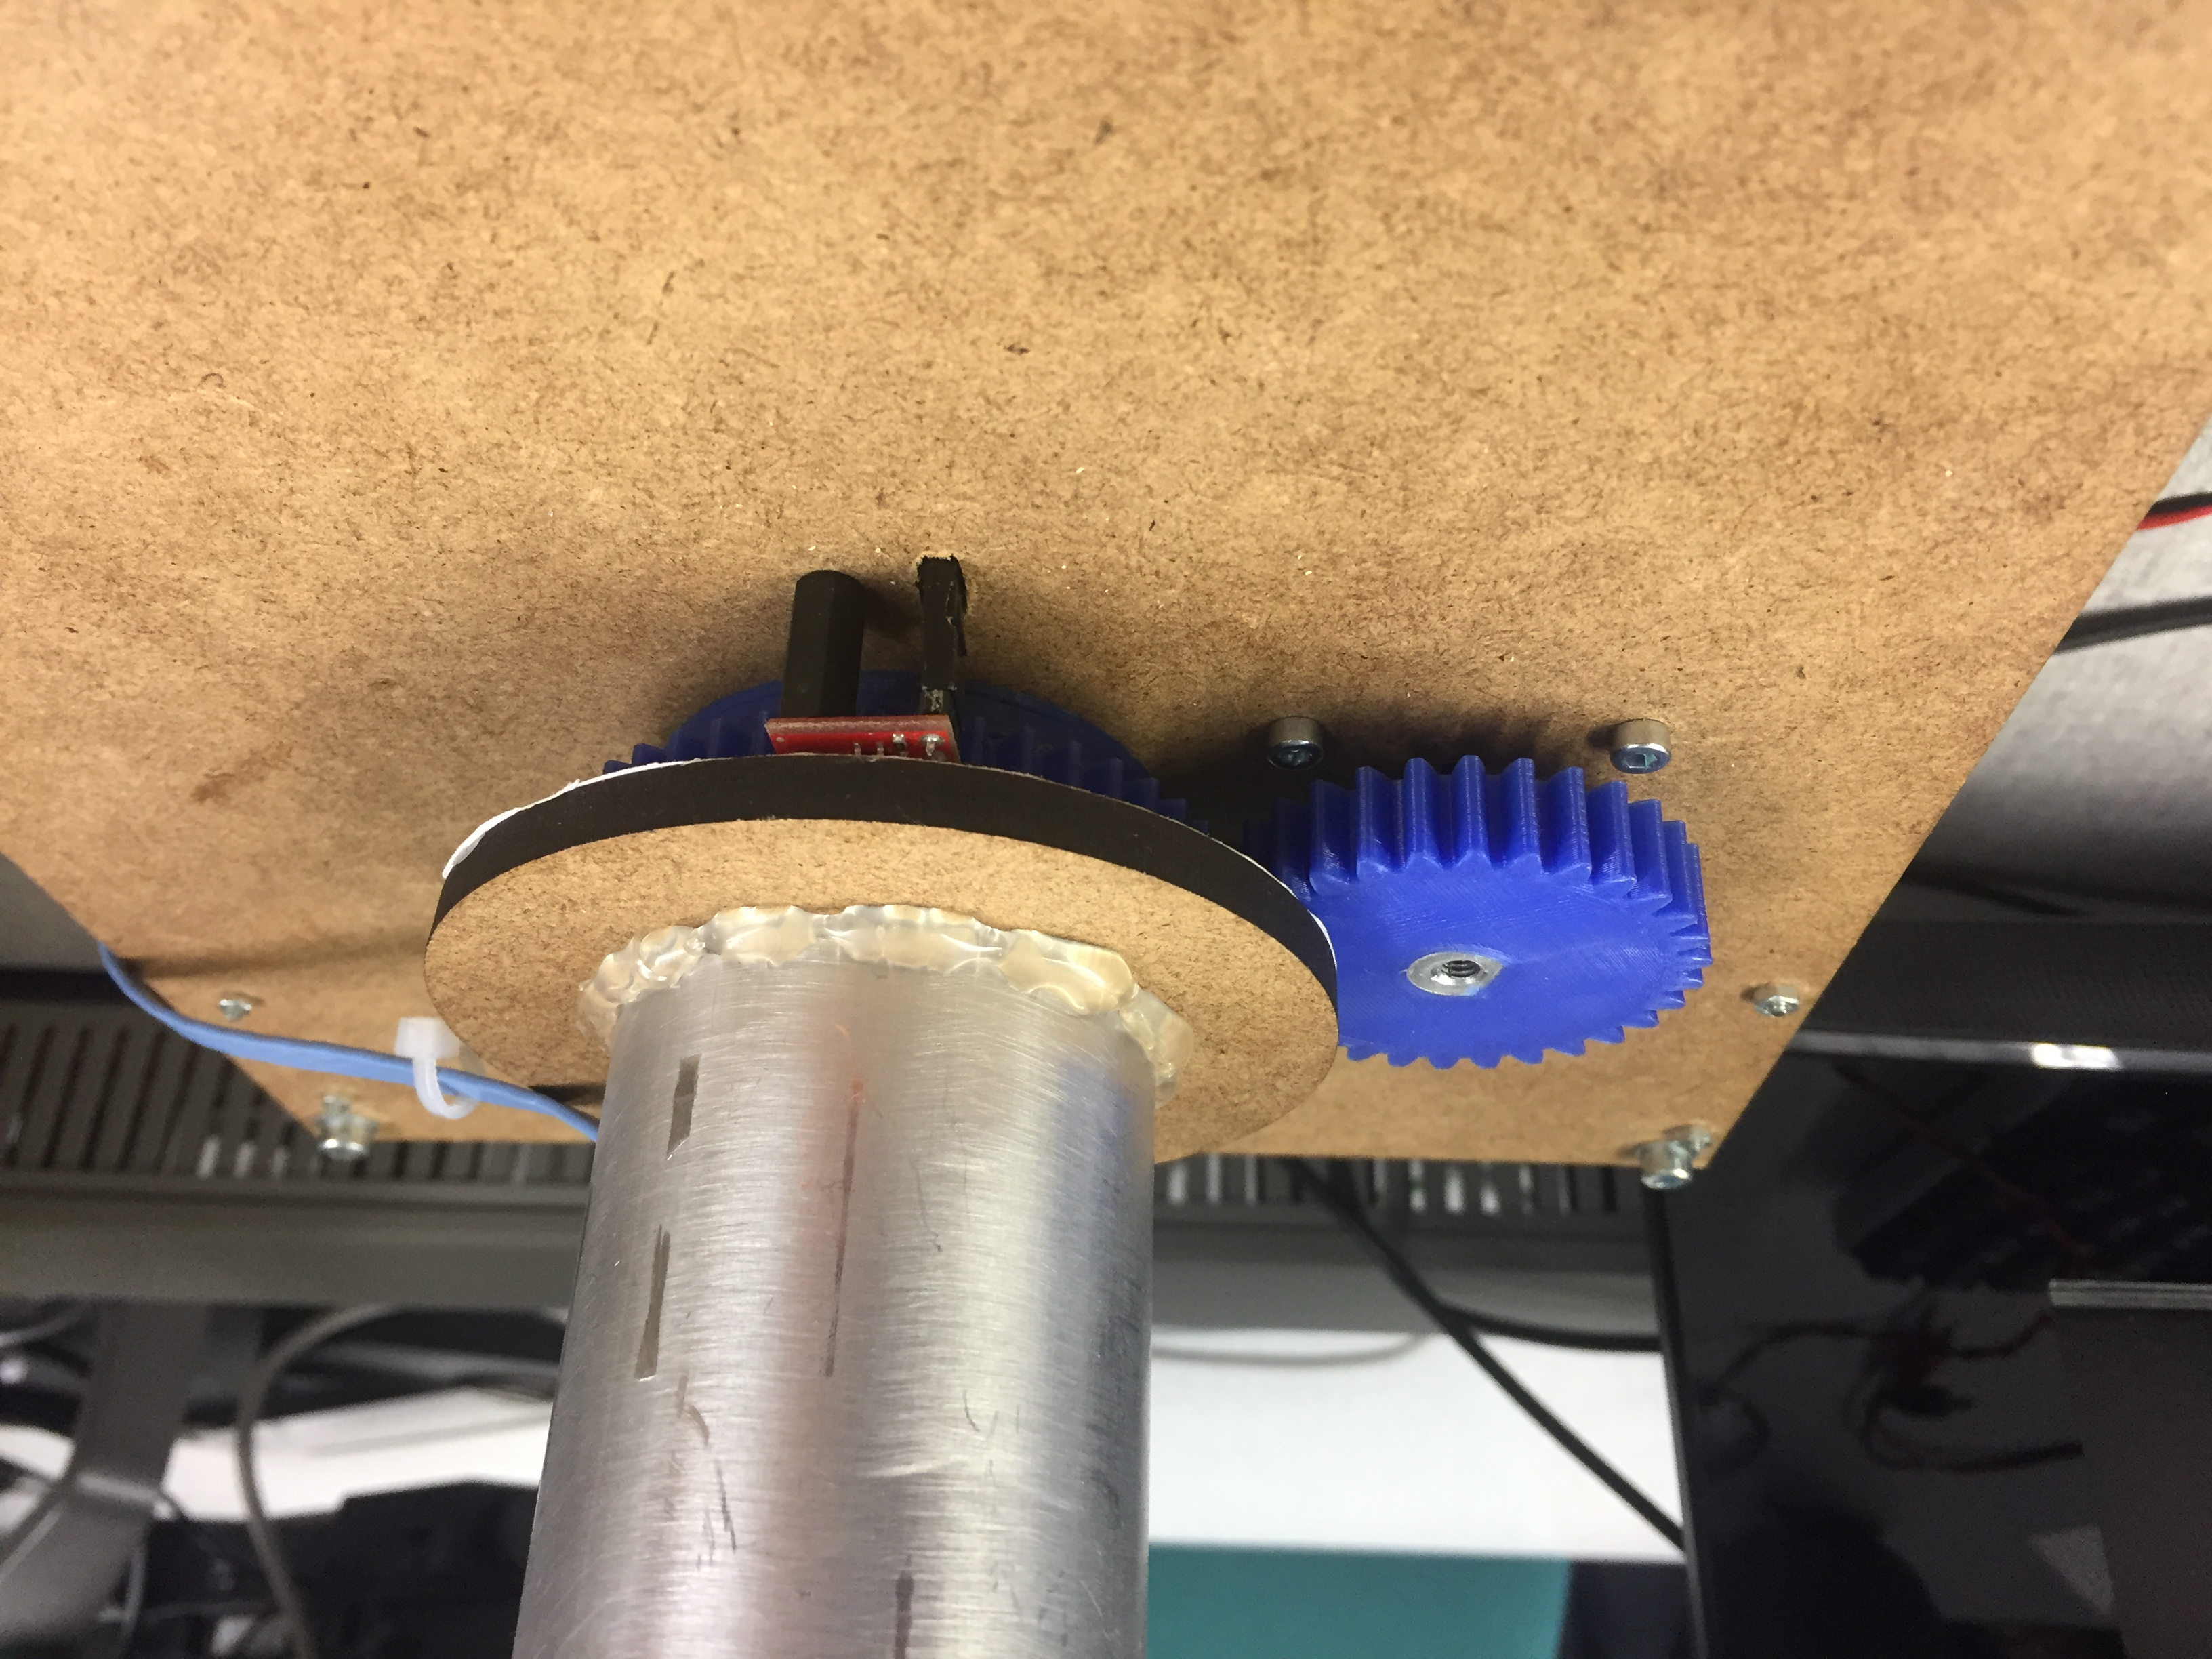
\includegraphics[angle=180,width=0.6\textwidth]{resources/Nullposition.jpg}
	\caption{Nullpunkterkennung mittels QRE 1113}
	\label{fig:Nullposition}
\end{figure} 

In der Konzeption wurde ein Gleichstrommotor der Marke Pololu für den Antrieb ausgewählt (siehe Unterkapitel \ref{subsec:Gleichstrommotor}). Während der Realisierung wurden sehr spät (Kalenderwoche 11) bedeutende Fehlverhalten des Motors festgestellt. Während den Leerlaufmessungen (Kalenderwoche 7) konnten keine Abweichungen der Encodersignale festgestellt werden. Nach dem Verbauen des Gleichstrommotors entsprachen die Encoder-Signale nicht den zu erwartenden Ergebnissen. Die Messwerte weichen mit bis zu 200 \ac{CPR}, welches umgerechnet ca. 36$^\circ$ ist vom Sollwert von 2248 ab. Dies verursacht unbrauchbare Resultate beim zusammenfügen der Punktwolken. Der Motor besitzt zusätzlich eine nicht nachvollziehbares Fehlverhalten. In einer Messung des Motorentreibers wurde ein fehlerfreies \ac{PWM} ausgemessen und auch die nötigen Strom- (1 Ampere) und Spannungswerte (12 Volt) verifiziert. Dennoch blockiert der Motor kurzzeitig willkürlich bei verschiedenen Drehpositionen. Dieses Fehlverhalten könnte auf ein internen Getriebedefekt zurück zu führen sein. Ursache für dieses Verhalten kann die Befestigungsschraube sein, welche bei der Montage hinein gedreht wurde. 

Aus den erwähnten Gründen wurde schnellst möglichst eine Alternative eruiert. Bei der Alternative handelt es sich um einen Schrittmotor der Marke Trinamic. Dieser Motor wurde aus Gründen der Verfügbarkeit und aus bereits bestehenden Kenntnissen über dessen Funktionsweise ausgewählt. Mit diesem Schrittmotor ist es möglich eine gleichmässige Umdrehungsgeschwindigkeit zu erreichen. 

Die Software wurde auf die neue Konfiguration angepasst und ist in Abschnitt \ref{subsec:Ansteuerung} erläutert. Es werden mittels 1/16 Schritte insgesamt 3200 Schritte für eine Umdrehung bei diesem Motor benötigt. Daraus ergibt sich mit der Übersetzung eine maximale Auflösung von $\frac{360^\circ}{1.5 * 3200}$ = 0.075$^\circ$. 
\todo{schrittverluste}

\section{Software}
\label{sec:SoftwareReal}
Wie bereits im Kapitel \ref{sec:Software} erläutert, wird durch das Velodyne Package ein grosser Teil der Aufgabenstellung bereits abstrahiert. Die einzelnen Aufgabenblöcke wurden nochmals unterteilt und sind in Abbildung \ref{fig:software_flow} dargestellt. Einerseits ist es nötig den Datenstream in einem weiteren Node zu empfangen und anderseits muss die Position ermittelt werden. Diese beiden Daten werden im Node \textit{/velodyne\_combined} zusammengefügt. Sobald die Daten kombiniert werden können, muss in einem weiteren Schritt die kombinierten Daten in einem Container gespeichert werden und bei Bedarf versendet.

\begin{figure}[H]
	\centering
	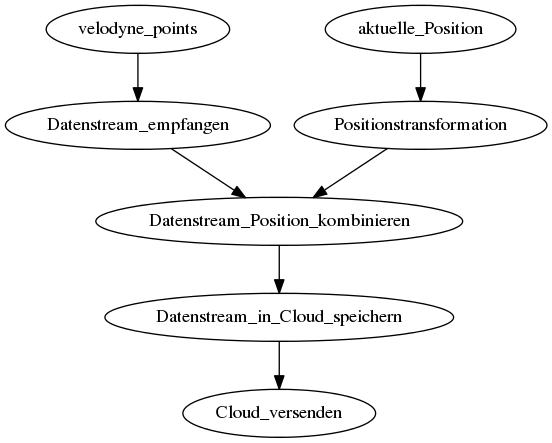
\includegraphics[width=0.5\textwidth]{resources/software_flow.png}
	\caption{Software Ablaufstruktur}
	\label{fig:software_flow}
\end{figure}  

Die Software wurde aufbauend konzipiert. Dabei wurde in einer ersten Phase das Empfangen und Weiterleiten mittels ROS \textit{Publisher und Subscriber} programmiert. In einem zweiten Schritt wurde die aktuelle Position mit den Daten kombiniert. In der letzte Phase wurde die Software mit dem Zusammenfügen der Datenpunkte zu einer Punktwolke erweitert. Wesentliche Codeausschnitte werden in den entsprechenden Unterkapiteln erläutert.

In Abbildung \ref{fig:rqt_graph_erweitert_2} ist mit \textcolor{red}{roter} Umrandung die Softwareerweiterung ersichtlich. Diese wurde in einem eigenen Package namens Laser\_3D erarbeitet, das im digitalen Anhang zu finden ist. 

\begin{figure}[H]
	\centering
	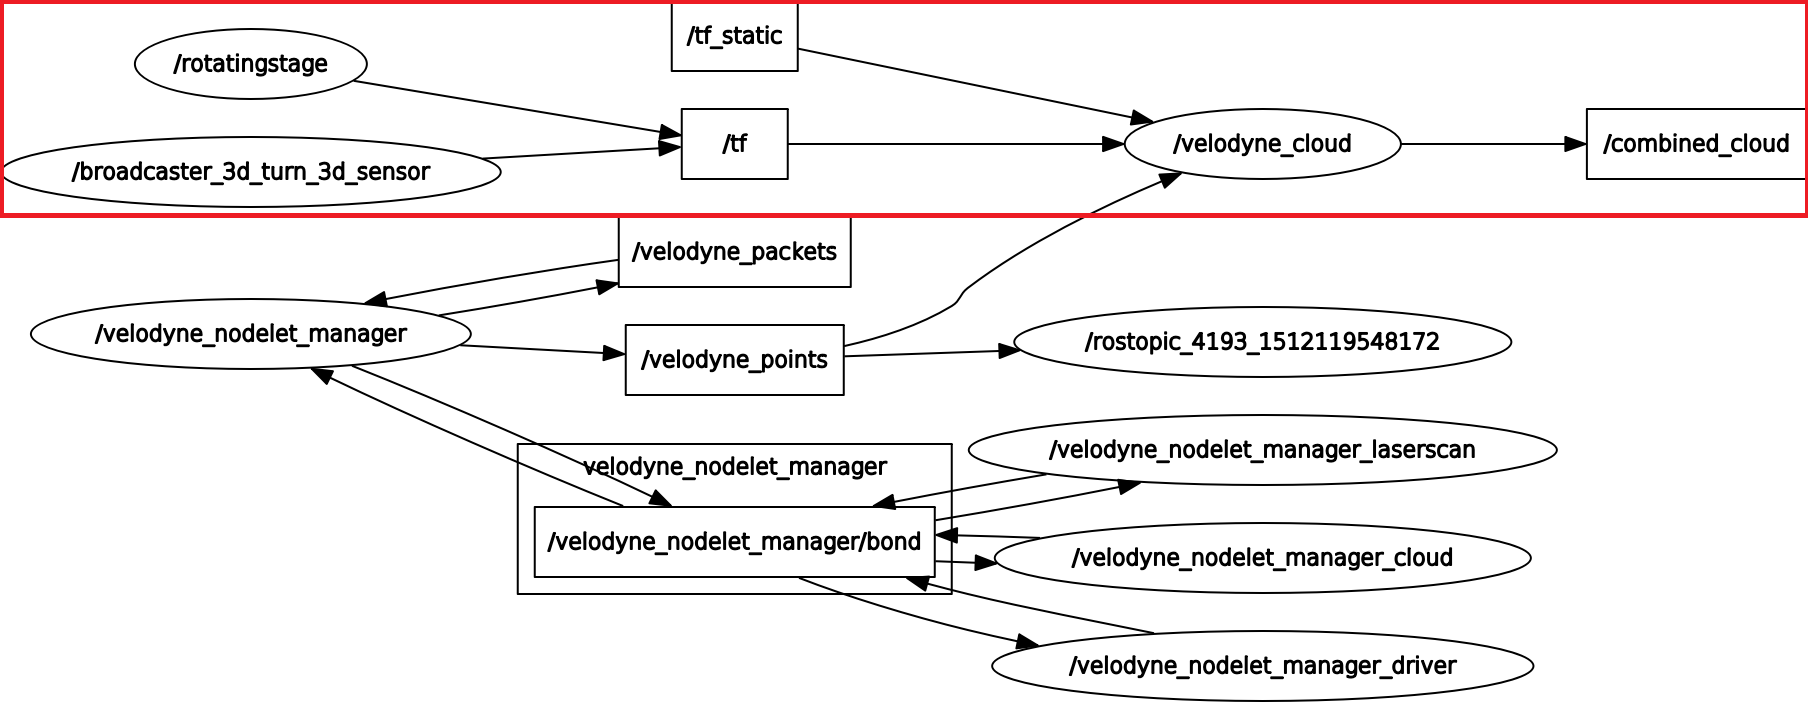
\includegraphics[width=0.75\textwidth]{resources/rqt_graph_erweitert_2.png}
	\caption{Softwareerweiterung mit Laser\_3D}
	\label{fig:rqt_graph_erweitert_2}
\end{figure} 
\subsection{Phase 1: Empfangen und Weitersenden}
\label{subsec:Phase2}
In dieser Phase wurden zu Beginn eine Programm implementiert, welche die Sensordaten (\textit{Messages}) empfängt und direkt wieder weiterleitet. Diese Funktion bietet das Grundgerüst für die weiteren Phasen. ROS bietet für diese Funtion zwei generische Klassen an. Der Publisher versendet Messages über sogenannte Topics, wie beispielsweise die \textit{velodyne\_points (vom Typ: velodyne\_msgs/PointCloud2)}. Subscriber können von Topics die Messages mittels einer Callback-Funktion an Variablen übergeben. Nachfolgend sind dazu die wesentlichsten Codeauschnitte wiedergegeben. \cite{pubsub} \todo{bilder schieben}

\begin{figure}[H]
	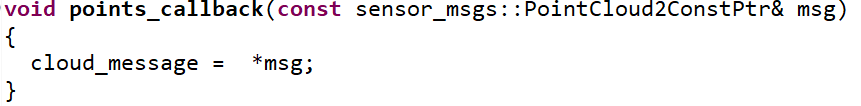
\includegraphics[width=0.62\textwidth]{resources/sourcecode/callback.png} \\
	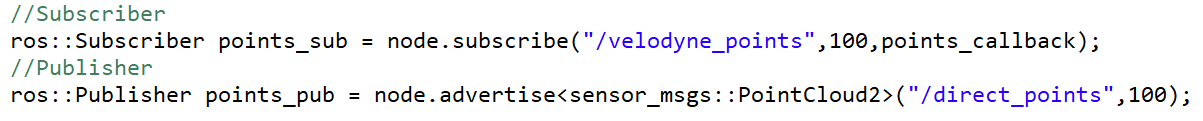
\includegraphics[width=0.9\textwidth]{resources/sourcecode/pubsub.png}
	%\caption{zusammengefügte mechanische Komponenten}
	\label{fig:pubsub}
\end{figure} 

\subsection{Phase 2: Positionstransformation}
\label{subsec:Phase}

Der empfangene Sensorstream kann mit Koordinatentransformation in die aktuelle Position des Drehturms transformiert werden. Es wird an dieser Stelle für die nachfolgenden Betrachtungen kurz Bezug zu Koordinatentransformation genommen \cite{Koordinaten}.
Es gelten für dreidimensionale Drehbewegungen folgende Matrizen:

$R_x(\phi ) =\begin{bmatrix}
	1&  0& 0\\ 
	0&  \cos\phi&  \sin\phi\\ 
	0&  -\sin\phi&  \cos\phi
\end{bmatrix}, R_y(\theta ) = \begin{bmatrix}
	\cos\theta&  0& -\sin\theta \\ 
	0&  1& 0\\ 
	\sin\theta &  0& \cos\theta 
\end{bmatrix}, R_z(\psi ) =\begin{bmatrix}
	\cos\psi& \sin\psi  & 0 \\ 
	-\sin\psi&  \cos\psi& 0 \\ 
	0&  0& 1
\end{bmatrix}$

Mit dem Rollwinkel $R_x(\phi)$ \textit{(engl. roll)}, Nickwinkel $R_y(\theta )$ \textit{(engl. pitch)} und Gierwinkel $R_y(\theta )$ \textit{(engl. yaw)} können in die 3 Freiheitsgrade beliebige Transformationen statisch oder dynamisch vorgenommen werden. Alternative können die Bewegungen mittels \ac{Quaternionen} angegeben werden. In Abbildung \ref{fig:rollpitchyaw} sind die Drehbewegungen mit den Achsen visualisiert.

\begin{figure}[H]
		\centering
	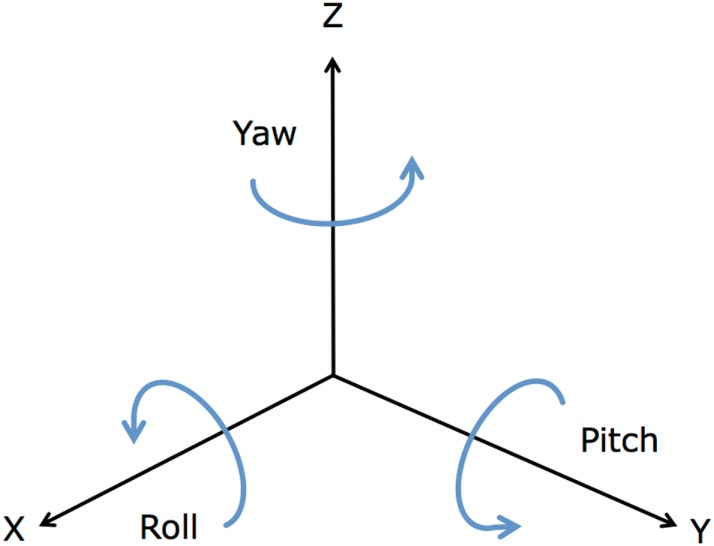
\includegraphics[width=0.3\textwidth]{resources/rollpitchyaw.png}
	\caption[{Roll-Pitch-Yaw mit X-Y-Z-Achsen}]{Roll-Pitch-Yaw mit X-Y-Z-Achsen}
	\label{fig:rollpitchyaw}
\end{figure} 

ROS bietet die Möglichkeit mehrere Koordinatensysteme miteinander zu verlinken und über die Klassen \textit{TF Broadcaster} und \textit{TF Listener} die aktuellen Positionen zu versenden und empfangen. In einem separaten Programmsegment \textit{rotatingstage} (siehe Abbildung \ref{fig:rqt_graph_erweitert_2}) wurde ein TF Broadcaster implementiert, welcher die aktuelle Ausrichtung des Drehturm versendet. Nachfolgender Codeauschnitte erläutern wesentliche Elemente. Es werden die Objekte \textit{TransformBroadcaster}, \textit{Transform} und \textit{Quaternion} verwendet, damit eine Bewegung erstellt wird.
\begin{figure}[H]
	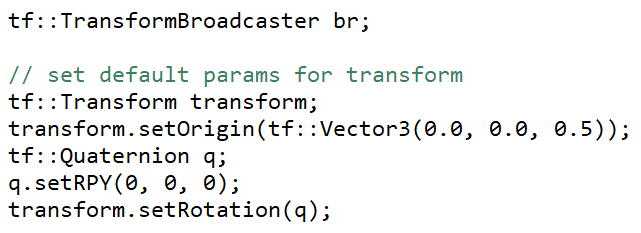
\includegraphics[width=0.5\textwidth]{resources/sourcecode/tf_broadcaster.png}	
\end{figure} 
Wird die aktuelle Position des Motors als Winkel phi übergeben und fortlaufend als Drehung in der Z-Achse (yaw) versendet, lassen sich die Koordinatenachsen verschieben. Da der Velodyne VLP-16 um -90$^\circ$ (270$^\circ$) geneigt ist, wurde die Transformation entsprechend gedreht (roll). Die versendete Transformation besitzt neben aktueller Position, einen Zeitstempel und die betreffenden Koordinatensysteme.
\begin{figure}[H]
	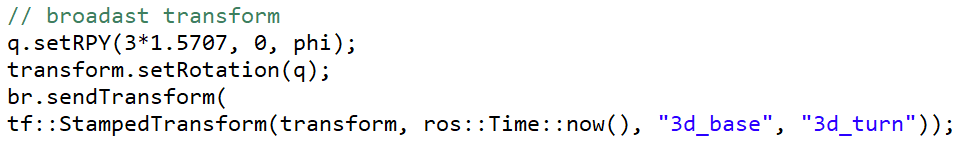
\includegraphics[width=0.8\textwidth]{resources/sourcecode/setrotation.png}	
\end{figure}
Der Node \textit{/velodyne\_combined} wurde mit einem TF Listener erweitert. Dieser ruft in einer lookup-Funktion die aktuelle Transformation ab und speichert diese in eine Variable.
\begin{figure}[H]
	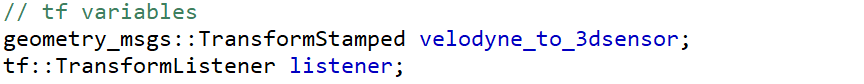
\includegraphics[width=0.7\textwidth]{resources/sourcecode/tf_listener.png}
	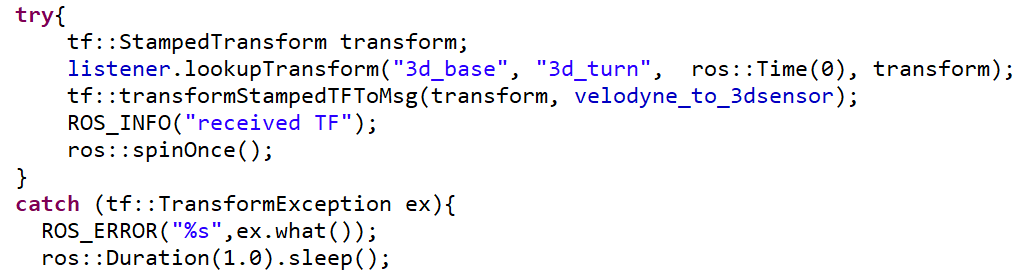
\includegraphics[width=0.7\textwidth]{resources/sourcecode/tf_update.png}		

\end{figure}
In Abbildung \ref{fig:koordinaten} sind die zwei Koordinatensysteme mit Rviz visualisiert. Die drehende Achse 3d\_turn, die mit der Achse 3d\_base verlinkt ist.
\begin{figure}[H]
	\centering
	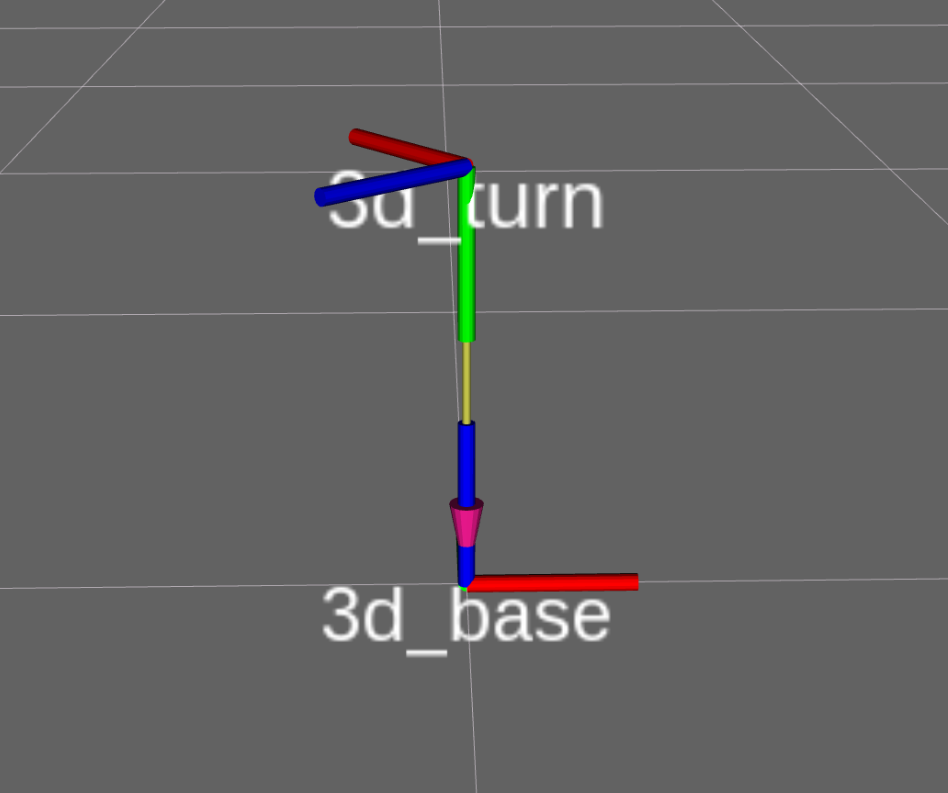
\includegraphics[width=0.5\textwidth]{resources/tf_rotation.PNG}
	\caption[dynamische Koordinatentransformation]{dynamische Koordinatensysteme}
	\label{fig:koordinaten}
\end{figure} 

\subsection{Phase 3: Punktwolke zusammenfügen}
\label{subsec:Phase3}
Während dieser Phase wurde eine \ac{Refactoring} gemacht und eine Klasse SubListener eingeführt. Ohne die Klasse verfügen mehrere Variablen nicht über den nötigen \ac{Scope}. In folgender Abbildung ist das Klassendiagramm mit entsprechenden Funktionen ersichtlich.

\begin{figure}[H]
	\centering
	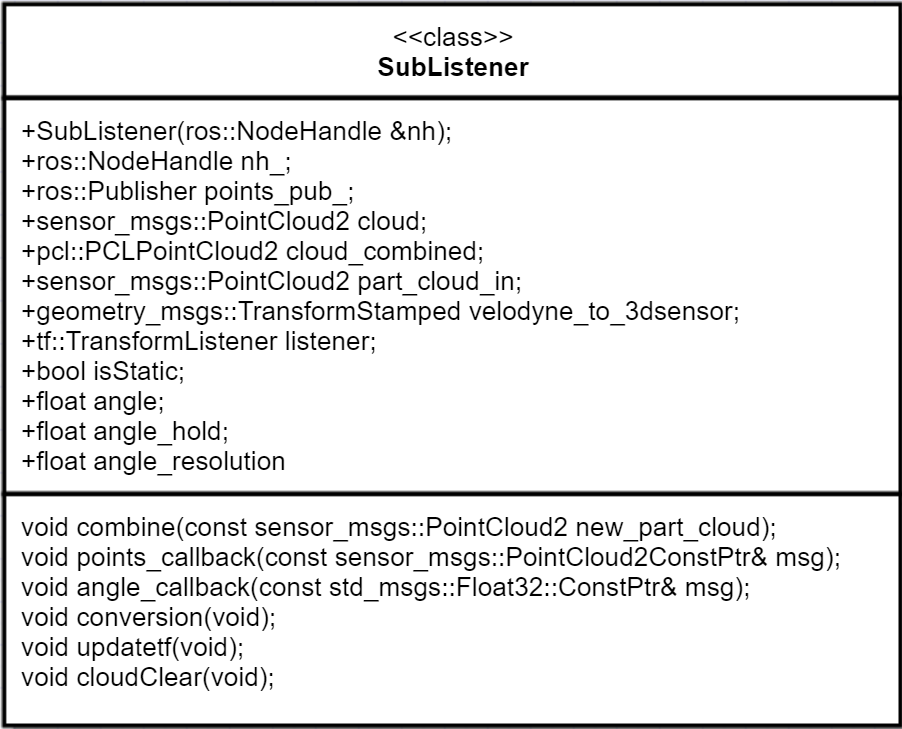
\includegraphics[width=0.5\textwidth]{resources/classdiagram.PNG}
	\caption[UML Klassendiagramm SuListener]{UML Klassendiagramm SubListener}
	\label{fig:classSubListener}
\end{figure} 

Die Klasse regelt alle Funktionen für das zusammenfügen der Punktwolken. Auf die detaillierte Erläuterungen wird in diesem Abschnitt verzichtet. 



In Abbildung \ref{fig:pointcloud_test} ist ein zusammengefügte Punktwolke ersichtlich. Durch entsprechende Parameteränderung lässt sich die Abtastung bei gegebener Umdrehungsgeschwindigkeit verändern.
 
\begin{figure}[H]
\centering
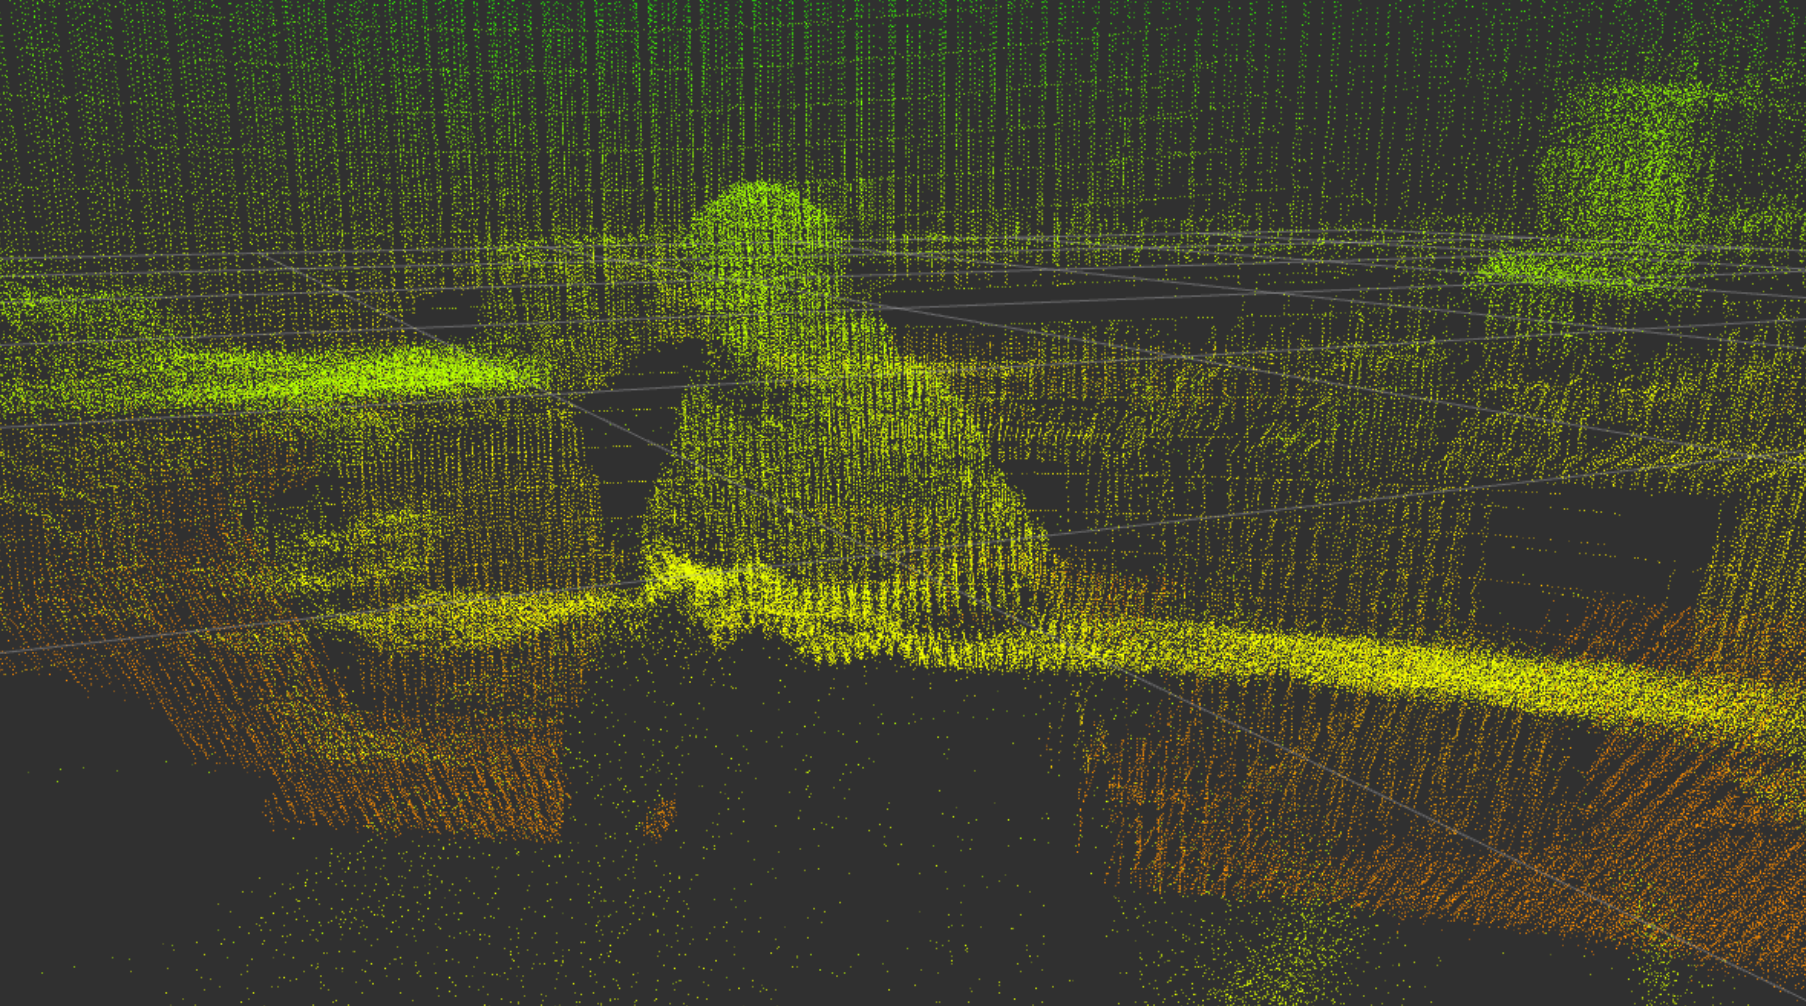
\includegraphics[width=1.0\textwidth]{resources/pointcloud_test.png}
\caption[Punktwolke einer Person bei Distanz 1m]{Punktwolke einer Person bei Distanz 1m}
\label{fig:pointcloud_test}
\end{figure}



In Abbildung \ref{fig:raumausmessung} ist ein Gesamtbild einer Punktwolke eines Raumes der Grösse 3 m x 15 m x 10m (HxBxT) ersichtlich. Die Abbildung zeigt die 

\begin{figure}[H]
	\centering
	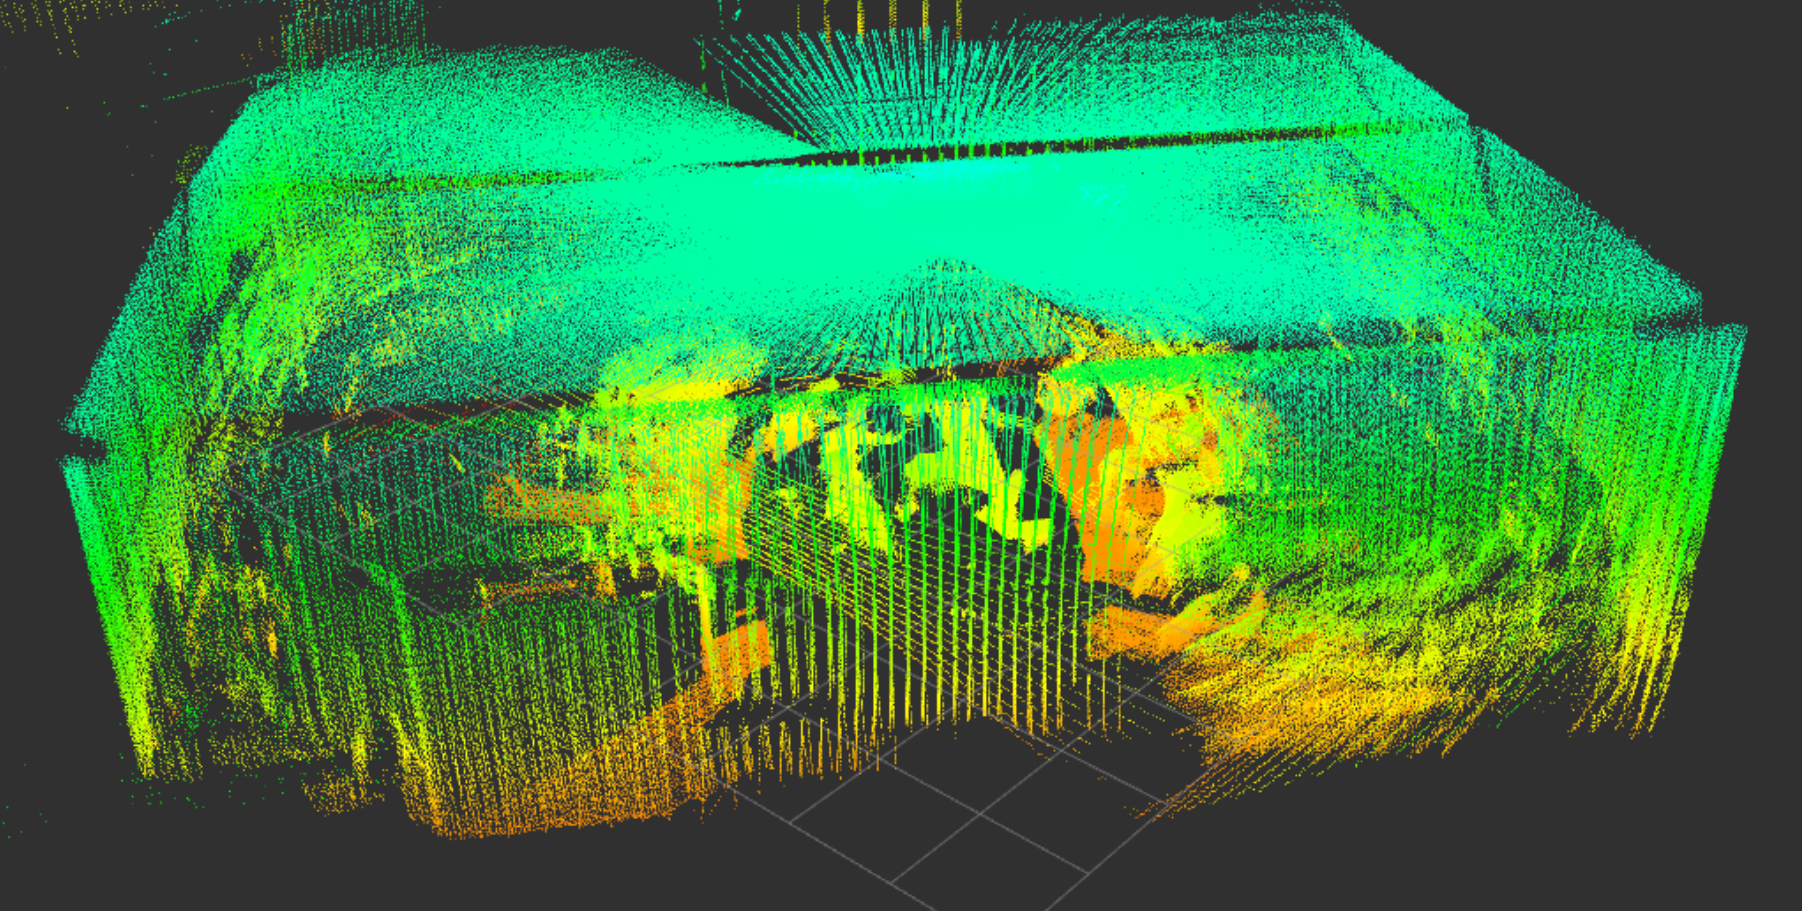
\includegraphics[width=1.0\textwidth]{resources/raumausmessung.png}
	\caption[zusammengefügte Punktwolken]{zusammengefügte Punktwolken}
	\label{fig:raumausmessung}
\end{figure}  



\subsection {Ansteuerung mittels GPIO}
\label{subsec:Ansteuerung}
\todo{gpio nach oben nehmen}
Wie bereits erwähnt wurde ein Schrittmotor der Marke Trinamic verwendet. Dieser wird über einen Motorentreiber A4988  angesteuert. Der Motorentreiber besitzt 


\section{Zwischenfazit}
\label{sec:ZwischenfazitReal}
ROS bietet viele Packages und Klassen, welche nützlich für die Softwareimplementation von Koordinatentransformation und Punktwolken sind. Die Freiheit von Open-Source bietet jedoch auch das Problem, dass die Kompatibilität von Packages nicht immer gewährleistet sind.  Anfänglich waren nru wenig Kenntnisse über die Koordinatentransformation vorhanden, daher verzögerte sich diese Softwarephase 2 erheblich. Es mussten einerseits die theoretischen Grundlagen verstanden werden und entsprechende Packages dazu evaluiert werden. Aufgrund z


